\thispagestyle{empty}
%\newgeometry{top=1.5cm, bottom=1.25cm, left=2cm, right=2cm}
%\fontfamily{rm}\selectfont

%\lhead{}
%\rhead{}
%\rfoot{}
%\cfoot{}
%\lfoot{}

\noindent 
%*****************************************************
%***** LOGO DE L'ED À CHANGER IMPÉRATIVEMENT *********
%*****************************************************
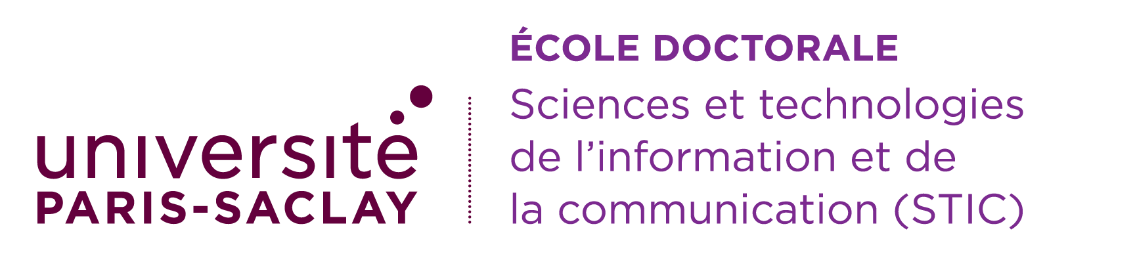
\includegraphics[height=2.45cm]{logos/logo_usp_STIC}
\vspace{1cm}
%*****************************************************
%\fontfamily{cmss}\fontseries{m}\selectfont

\begin{mdframed}[linecolor=Prune,linewidth=1,nobreak=false]
\footnotesize	
\onehalfspacing
\textbf{Titre: Traduction Automatique Neuronale Multi-domaines} \\
\noindent \textbf{Mots clés:} Traduction neuronale, Adaptation au domaine, Apprentissage multi-tâche
\vspace{-.1cm}
\begin{multicols}{2}
\noindent \textbf{Résumé:} Aujourd'hui, les systèmes de traduction automatique neuronale (NMT) constituent des systèmes de pointe en traduction automatique (TA). Cependant, ces modèles de traduction nécessitent des données d'entraînement relativement volumineuses et ont de la difficulté à traduire des textes de domaine spécifique. Un domaine peut être constitué de textes d'un sujet particulier ou de textes écrits dans un but particulier. Bien que les systèmes NMT puissent être adaptés pour une meilleure qualité de traduction dans un domaine cible étant donné un corpus de train représentatif, cette technique a des effets secondaires négatifs, notamment une fragilité contre des exemples hors domaine et un "oubli catastrophique" des domaines précédents représentés dans les données d'entraînement. De plus, un système de traduction doit faire face à de nombreux domaines possibles dans des applications réelles, ce qui rend impraticable le "un domaine un modèle". Une solution prometteuse consiste à construire des systèmes NMT multi-domaines formés à partir des données de nombreux domaines et adaptés à plusieurs domaines cibles. Il y a deux motivations. Premièrement, les grands corpus de trains améliorent la généralisation du système NMT. Deuxièmement, les textes d'un domaine peuvent être utiles pour adapter un modèle NMT à un domaine similaire. La pénurie des données et l'effet de transfert positif hypothétique sont également deux raisons principales pour le développement des systèmes NMT multilingues. Maintenir plusieurs systèmes de traduction automatique bilingues nécessite de nombreuses ressources matérielles, car le nombre de paires de langues augmente de façon quadratique avec l'augmentation du nombre de langues. Les systèmes NMT multi-domaines et multilingues sont essentiels pour économiser des ressources pour l'industrie TA et améliorer la qualité du service TA. Cette thèse unifie d'abord l'adaptation de domaine et l'adaptation multi-domaine dans un cadre mathématique. De plus, nous passons en revue la littérature sur l'adaptation aux (multi-)domaines à travers une approche structurelle en montrant quatre cas principaux et en associant les méthodes proposées à chaque cas d'application. Deuxièmement, nous proposons une nouvelle évaluation multicritères des approches multi-domaines. Nous soulignons les exigences d'un système multi-domaines et réalisions une comparaison exhaustive d'un large ensemble de méthodes. Nous proposons également de nouvelles méthodes pour l'adaptation aux multi-domaines, y compris les plongements de mot parcimonieux, les couches parcimonieux et les adaptateurs résiduels, qui sont relativement légers et capables d'adapter un NMT modèle aux nombreux domaines. Pour équilibrer l'hétérogénéité des données d'entraînement, nous explorons et étudions les techniques à l'échantillonnage dynamique des données, qui adaptent de manière itérative la distribution de l'entraînement à une distribution de test prédéterminée. Enfin, nous nous intéressons aux approches de traduction avec des contextes augmentés, qui réutilisent des mémoires de traduction similaires pour améliorer la prédiction d'une phrase. Nous analysons et comparons plusieurs méthodes de cette ligne et démontrons qu'elles conviennent pour adapter notre système NMT à un domaine inconnu au détriment de coûts de calcul supplémentaires.
\end{multicols}
\end{mdframed}

\vspace{8mm}

\begin{mdframed}[linecolor=Prune,linewidth=1]
\footnotesize	
\onehalfspacing
\textbf{Title:} Multi-domain Neural Machine Translation\\
\noindent \textbf{Keywords:} Neural machine translation, Domain adaptation, multi-task learning
\begin{multicols}{2}
\noindent \textbf{Abstract:} Today, neural machine translation (NMT) systems constitute state-of-the-art systems in machine translation. However, such translation models require relatively large train data and struggle to handle a specific domain text. A domain may consist of texts from a particular topic or texts written for a particular purpose. While NMT systems can be adapted for better translation quality in a target domain given a representative train corpus, this technique has adverse side-effects, including brittleness against out-of-domain examples and "catastrophic forgetting" of previous domains represented in the train data. Moreover, one translation system must cope with many possible domains in real applications, making the "one domain one model" impractical. A promising solution is to build multi-domain NMT systems trained from many domains and adapted to multiple target domains. The rationale behind this is twofold. First, large train corpora improve the generalization of the NMT system. Secondly, texts from one domain can be valuable for adapting an NMT model to a similar domain. The scarcity of data and the hypothetical positive transfer effect are also two main reasons for building multilingual NMT systems. Maintaining multiple bilingual MT systems requires lots of hardware resources as the number of language pairs grows quadratically with the increasing number of languages. Both multi-domain and multilingual NMT systems are essential for saving resources for the MT industry and improving the quality of the MT service.

This thesis first unifies domain adaptation and multi-domain adaptation in one mathematical framework. In addition, we review the literature of (multi-)domain adaptation through a structural approach by pointing out four principal cases and matching previous methods to each application case. Secondly, we propose a novel multi-criteria evaluation of multi-domain approaches. We point out the requirements for a multi-domain system and perform an exhaustive comparison of a large set of methods. We also propose new methods for multi-domain adaptation, including sparse word embeddings, sparse layers, and gated residual adapters, which are cheap and able to handle many domains. To balance the heterogeneity in the train data, we explore and study techniques relating to dynamic data sampling, which iteratively adapt the train distribution to a pre-determined testing distribution. Finally, we are interested in context augmented translation approaches, which reuse similar translation memories to improve the prediction of a sentence. We carefully analyze and compare several methods in this line and demonstrate that they are suitable for adapting our NMT system to an unknown domain at the expense of additional computational costs.
\end{multicols}
\end{mdframed}